\documentclass[../main.tex]{subfiles}

\begin{document}
\section{Introduction to astrophysics and satellite tracking}
\subsection{The two body problem}
\subsubsection{Trajectory equation}
We are interested in understanding the dynamics of a spacecraft in orbit around the Earth. These dynamics are governed by Newton's second law of motion, which assuming that both the Earth and the spacecraft are point masses (see \cref{sec:force} for a more realistic model), can be written as
\begin{equation}
  \label{eq:Newton}
  \ddot{\vf{r}}=-\frac{GM_{\oplus}}{r^2}\vf{e}_r
\end{equation}
where $\vf{r}$ is the position vector (also called \emph{radius vector}) of the spacecraft with respect to the Earth, $r:=\norm{\vf{r}}$, $\vf{e}_r=\frac{\vf{r}}{r}$ is the unit vector in the direction of $\vf{r}$, $M_{\oplus}\simeq 5.972\times 10^{24}\ \kg$ is the mass of the Earth, and $G\simeq 6.674\times 10^{-11}\ \m^3\cdot \kg^{-1}\cdot\s^{-2}$ is the gravitational constant. Note that the minus sign is due to the fact that the gravitational force is attractive, i.e. pointing towards the Earth.
Here and along the document the notation $\ddot{\vf{r}}$ means that the derivative is taken with respect to time.
Cross-multiplying \cref{eq:Newton} by $\vf{r}$, we obtain
\begin{equation}
  \dv{(\vf{r}\times \dot{\vf{r}})}{t}=\dot{\vf{r}}\times \dot{\vf{r}}+\vf{r}\times\ddot{\vf{r}}=-\frac{GM_{\oplus}}{r^3}(\vf{r}\times \vf{r})=0
\end{equation}
Hence $\vf{r}\times \dot{\vf{r}}=:\vf{h}$ is constant. The physical intuition behind this is that the motion of the spacecraft around the Earth is confined to a plane, which is called the \emph{orbital plane} because the position $\vf{r}$ and velocity $\vf{r}$ are always perpendicular to $\vf{h}$, which is the normal vector to the orbital planes and it relates to the \emph{angular momentum} of the spacecraft.

We are interested now in what kind of curves may be described by a body orbiting the other one. That is, we want somehow isolate $\vf{r}$ (or $r$) from \cref{eq:Newton}. In order to simplify the notation we will denote $\mu:=GM_{\oplus}$.
\begin{proposition}[Kepler's first law]
  \label{prop:two-body}
  The motion of a body orbiting another one is described by a conic. Hence it can be expressed in the form:
  \begin{equation}
    \label{eq:two-body}
    r(t)=\frac{p}{1+e\cos (\nu(t))}
  \end{equation}
  for some parameters $p$ and $e$.
\end{proposition}
\begin{proof}
  Cross-multiplying \cref{eq:Newton} by $\vf{h}$ we obtain
  \begin{equation}
    \dv{(\dot{\vf{r}}\times\vf{h})}{t}=\ddot{\vf{r}}\times\vf{h}=-\frac{\mu}{r^3}\vf{r}\times\vf{h}=-\frac{\mu}{r^3}\vf{r}\times(\vf{r}\times \dot{\vf{r}})=-\frac{\mu}{r^3}[(\vf{r}\cdot{\vf{r}})\dot{\vf{r}}-(\vf{r}\cdot\dot{\vf{r}})\vf{r}]
  \end{equation}
  where we have used \cref{prop:triplecross}. Now note that:
  \begin{equation}
    \dv{}{t}\left(\frac{\vf{r}}{r}\right)=\frac{\dot{\vf{r}}}{r}-\frac{\dot{r}}{r^2}\vf{r}= \frac{1}{r^3}[(\vf{r}\cdot{\vf{r}})\dot{\vf{r}}-(\vf{r}\cdot\dot{\vf{r}})\vf{r}]
  \end{equation}
  because $2r\dot{r}=\dv{(r^2)}{t}=\frac{(\vf{r}\cdot\vf{r})}{t}=2\vf{r}\cdot\dot{\vf{r}}$\footnote{Bear in mind that in general $\dot{r}\ne\norm{\dot{\vf{r}}}$. Indeed, if $\beta$ denotes the angle between $\vf{r}$ and $\dot{\vf{r}}$ we have that $\dot{r}=\norm{\dot{\vf{r}}}\cos\beta$. In particular $\dot{r}$ may be negative.}. Thus:
  \begin{equation}
    \dv{(\dot{\vf{r}}\times\vf{h})}{t}=\mu \dv{}{t}\left(\frac{\vf{r}}{r}\right)
  \end{equation}
  Integrating with respect to the time yields
  \begin{equation}
    \dot{\vf{r}}\times \vf{h}=\frac{\mu}{r}\vf{r}+\vf{B}
  \end{equation}
  where $\vf{B}\in\RR^3$ is the constant of integration. Now dot-multiplying this last equation by $\vf{r}$ and using that $\vf{u}\cdot(\vf{v}\times\vf{w})=(\vf{u}\times\vf{v})\cdot\vf{w}$ $\forall\vf{u},\vf{v},\vf{w}\in\RR^3$ we obtain
  \begin{equation}
    h^2=\vf{h}\cdot\vf{h}=(\vf{r}\times\dot{\vf{r}})\cdot\vf{h}=\vf{r}\cdot(\dot{\vf{r}}\times\vf{h})=\frac{\mu}{r}\vf{r}\cdot\vf{r}+\vf{r}\cdot\vf{B}=\mu r+rB\cos\nu
  \end{equation}
  where $h:=\norm{\vf{h}}$, $B:=\norm{\vf{B}}$ and $\nu$ denotes the angle between $\vf{r}$ and $\vf{B}$. Rearranging the terms we obtain finally the equation of a conic
  \begin{equation}\label{eq:r_conic}
    r=\frac{h^2/\mu}{1+(B/\mu)\cos(\nu)}
  \end{equation}
  with $p:=h^2/\mu$ and $e:=B/\mu$.
\end{proof}
Among the range of values that can $r$ take, we are particularly interested in the minimum and maximum values, $r_\mathrm{min}$ and $r_\mathrm{max}$, that can be attained. Is easy to see that these are given by
\begin{equation}
  r_\mathrm{min}=\frac{p}{1+e}\qquad\text{and}\qquad r_\mathrm{max}=
  \begin{cases}
    \displaystyle\frac{p}{1-e} & e<1     \\
    \infty                     & e\geq 1
  \end{cases}
\end{equation}
The points on the orbit of such distances are attained are called \emph{apoapsis} and \emph{periapsis} respectively. The line connecting both points is called \emph{line of apsides}, and the half of the distance between them is the \emph{semi-major axis} and is denoted by $a$:
\begin{equation}\label{eq:semi-major_axis}
  a:=\frac{r_\mathrm{max}+r_\mathrm{min}}{2}=
  \begin{cases}
    \displaystyle\frac{p}{1-e^2} & e<1     \\
    \infty                       & e\geq 1
  \end{cases}=
  \begin{cases}
    \displaystyle\frac{h^2}{\mu(1-e^2)} & e<1     \\
    \infty                              & e\geq 1
  \end{cases}
\end{equation}
because we have considered the reference frame of \cref{fig:conics_cartesian} and so the line of apsides crosses the origin. Finally the angle $\nu$ is called \emph{true anomaly}.
\begin{definition}
  Let $\vf{r}(t)$, $\vf{r}(t+k)$ be the positions of the small body at times $t$, $t+k$ respectively. Let $A(t)$ be the area swept by the radius vector $\vf{r}(t)$ in the time interval $[0,t]$. We define the \emph{areal velocity} as $\dv{A(t)}{t}$.
\end{definition}
\begin{proposition}[Kepler's second law]
  The areal velocity remains constant.
\end{proposition}
\begin{proof}
  Recall that the area of a parallelogram generated by two vectors $\vf{u},\vf{v}\in\RR^3$ is given by $\norm{\vf{u}\times\vf{v}}$. Thus, approximating the area $A$ by half of the parallelogram generated by $\vf{r}(t)$ and ${\vf{r}}(t+k)$ we obtain
  \begin{multline}\label{eq:areal_velocity}
    \dv{A(t)}{t}=\lim_{k\to 0}\frac{A(t+k)-A(t)}{k}=\lim_{k\to 0}\frac{\norm{\vf{r}(t)\times\vf{r}(t+k)}}{2k}=\lim_{h\to 0}\frac{\norm{\vf{r}(t)\times(\vf{r}(t+k)-\vf{r}(t))}}{2k}=\\
    =\frac{\norm{\vf{r}(t)\times\dot{\vf{r}}(t)}}{2}=\frac{h}{2}
  \end{multline}
  where the penultimate equality is because the cross product is continuous and linear.
\end{proof}

From now one we will suppose that the orbits are ellipses, which is the main case of interest.
\subsubsection{Kepler's equation}
So far we have been able to describe the geometry of motion of a body orbiting another one. However, we have not been concerned about the specific position of the body as a function of time. That is how to obtain $\nu(t)$ at each instant of time. In order to do this, we may think the area $A$ as a function of $\nu$, that measures the area swept by the radio vector from an initial instant $\nu_0$. Thus, from differential calculus we know that:
\begin{equation}
  A(\nu)=\int_{\nu_0}^{\nu}\int_{0}^{r(\theta)}r\dd{r}\dd{\theta}=\int_{\nu_0}^{\nu}\frac{r(\theta)^2}{2}\dd{\theta}\implies\dv{A}{\nu}=\frac{r^2}{2}
\end{equation}
And using the chain rule and \cref{eq:areal_velocity} we obtain that:
\begin{equation}\label{eq:areal_velocity_nu}
  \frac{h}{2}=\dv{A}{t}=\dv{A}{\nu}\dv{\nu}{t}=\frac{r^2}{2}\dot\nu
\end{equation}
So from \cref{eq:r_conic,eq:areal_velocity_nu} we get the following differential equation that must satisfy $\nu$:
\begin{equation}
  \dot\nu=\frac{h}{r^2}=\frac{h}{p^2}{(1+e\cos\nu)}^2
\end{equation}
which, when integrated with respect to the time, lead us to an elliptic integral. Our goal in this section is to find an easier way to compute exact position of the satellite ate each instant of time. This will lead us to the so-called \emph{Kepler's equation}. For this purpose we are forced to introduce a new parameter, $E$, called \emph{eccentric anomaly}. It is defined as the angle between the line of apsides and the line passing through the center of the ellipse and the point at the circle which is just above the position of the satellite (see \cref{fig:kepler_eq} for a better understanding).
\begin{figure}[ht]
  \centering
  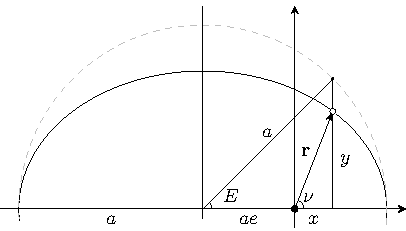
\includegraphics[width=0.5\textwidth]{Images/kepler_eq.pdf}
  \caption{Ellipse orbit of the satellite together with an auxiliary circle of radius $a$ needed to define the eccentric anomaly.}
  \label{fig:kepler_eq}
\end{figure}

Clearly the position of the satellite is determined by $x=r\cos\nu$, $y=r\sin\nu$. But we would like to find an expression of $x$ and $y$ in terms of $E$ rather than $\nu$. To do this note that $a\cos E=ae+x$, so:
\begin{equation}\label{eq:eccentricX}
  x=a(\cos E-e)
\end{equation}
And so we can get an expression of $r$ in terms of $E$ by solving the equation:
\begin{equation}\label{eq:eccentricr}
  r=\frac{p}{1+e\cos \nu}=\frac{a(1-e^2)}{1+e\frac{x}{r}}=\frac{ra(1-e^2)}{r+ae(\cos E-e)}\implies r= a(1-e\cos E)
\end{equation}
Finally from \cref{eq:eccentricX,eq:eccentricr} we get:
\begin{equation}
  y^2=r^2-x^2=a^2(1-e^2){(\sin E)}^2\implies y=a\sqrt{1-e^2}\sin E
\end{equation}
Expressing now the areal velocity $h$ as a function of $E$ we have:
\begin{align}
  h & =x\dot{y}-y\dot{x}                                                           \\
    & =a^2(\cos E-e)\sqrt{1-e^2}(\cos E)\dot{E}+a^2{(\sin E)}^2\dot{E}\sqrt{1-e^2} \\
    & =a^2\sqrt{1-e^2}\dot{E}(1-e\cos E)
\end{align}
From \cref{eq:semi-major_axis} we know that $h=\sqrt{\mu a(1-e^2)}$. Thus substituting this in the latter equation we deduce that $E$ must satisfy the following differential equation:
\begin{equation}
  \dot{E}(1-e\cos E)=\sqrt{\frac{\mu}{a^3}}=:n
\end{equation}
where $n$ is called the \emph{mean motion}. Integrating this equation with respect to time yield the \emph{Kepler's equation}:
\begin{equation}
  E(t)-e\sin E(t)=n(t-t_0)
\end{equation}
where $t_0$ is the time at which $E$ vanishes. Using the reference frame of \cref{fig:kepler_eq} this corresponds at the time at which the satellite is at the perigee. The value $M:=n(t-t_0)$ is called \emph{mean anomaly}.

Kepler's equation is the key to solve the problem of finding the position of the satellite at each instant of time. Later on we will discuss techniques to solve this equation for $E$ knowing $e$ and $M$.
\subsection{Time and reference systems}
\end{document}